\section{Front geometries, time windows, and large droplets}
\label{sec:sfronts}

A strip of the active phase next to the absorbing state grows on one side of
the transition and shrinks on the other. The broad survey places reversal
near $q=0.04592$; the longer measurements below refine this location.
Behind a retreating front, the interior retains a substantial interface-site
fraction ($\iota_{\rm in}\simeq0.71$ at $q\simeq0.0436$, compared with about
0.76 near reversal). The active region is therefore invaded coherently before
it disappears. At a continuous transition the asymptotic active density would
instead vanish at the boundary. A finite-time retreating interface alone
does not distinguish these cases; we compare it with bulk and nucleation
measurements below. Front reversal also locates phase competition in the
four-species alliance model~\cite{szabo2004} and in spatial bistable
systems~\cite{durrett1994,durrett2009}.

In nonequilibrium systems, the reversal point can depend on front orientation.
Between the extreme crossings, a window of generic coexistence can open in
which sufficiently large droplets of either phase shrink by
faceting~\cite{toom1980,bennett1985,wang2015}. We compare bands with normals
$(1,0)$, $(2,1)$, and $(1,1)$, at $0^\circ$, $26.6^\circ$, and $45^\circ$
to the axes. Figure~\ref{fig:orient} shows the broad survey at $p=0.1$, $1/2$,
and $0.9$, with $L=4096$, eight seeds per point, and $T=2\times10^5$.
The outermost threshold crossings of the smoothed profile locate the band;
interior holes do not terminate this envelope. The smoothing length is nine
lattice spacings in the physical normal direction for every orientation.

At $p=1/2$, local interpolation between the two points bracketing reversal,
using $t\ge2\times10^4$, gives $q^*=0.045919$, 0.045911, and 0.045923 for
these three normals. Their conditional 95\% seed-bootstrap intervals are
$[0.045912,0.045927]$, $[0.045902,0.045921]$, and
$[0.045912,0.045933]$, respectively. Time windows, threshold levels, and fit
curvature are varied separately to assess systematic sensitivity. Several
straight-line fits across the entire sampled range have significant lack of
fit; their formal errors are not used as the full uncertainty of a crossing.
The broad survey finds only small orientation differences, but does not by
itself establish a unique orientation-independent transition point. It
constrains a broad generic-coexistence window of the type observed in
Ref.~\cite{wang2015} and motivates the finer comparisons below.

\begin{figure*}
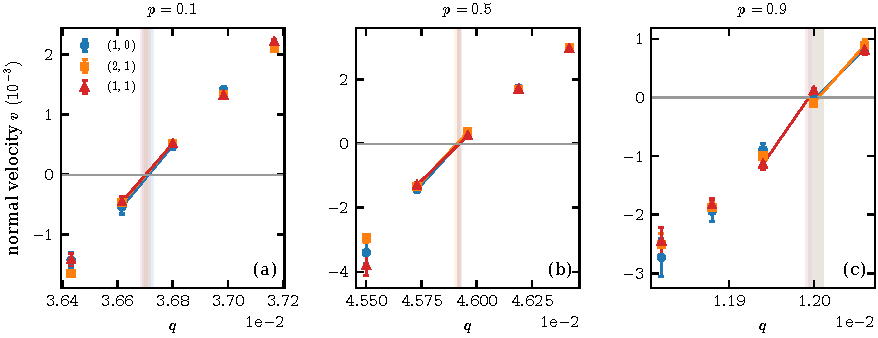
\includegraphics[width=\textwidth]{figs/fig_orient}
\caption{Normal velocity of a band of the active phase against the absorbing state, for normal
directions $(1,0)$, $(2,1)$, and $(1,1)$, at $p = 0.1$, $1/2$, and $0.9$; $L = 4096$, $T = 2\times10^5$,
eight seeds per point, velocity from the width of the band tracked along its normal for
$t\ge2\times10^4$. The horizontal coordinate is the actual probability $q$.
Lines interpolate the two seed-averaged velocities bracketing reversal;
shaded bands are conditional 95\% run-bootstrap intervals for the crossing.
Smoothing uses the same physical normal length for all orientations.
Farther below reversal the strip can nucleate absorbing domains internally,
so the broad-range velocity curve need not be linear.}
\label{fig:orient}
\end{figure*}

The fine-grid campaign extends these tests to $L=8192$ and 16384 and
$T=2\times10^6$ (Fig.~\ref{fig:gpu_fronts}). At $L=8192$, all five
probabilities and all three orientations have four completed independent
runs. Over $10^6\le t\le2\times10^6$, the local crossings are
0.0459387, 0.0459396, and 0.0459398 for normals $(1,0)$, $(2,1)$,
and $(1,1)$, respectively. Their spread is $1.0\times10^{-6}$, with a
conditional 95\% bootstrap upper value of $1.02\times10^{-5}$; simultaneous
pairwise intervals include zero. Varying the profile threshold from 0.2
to 0.5 gives crossings spanning 0.0459371--0.0459442 at this size and
window. At $L=16384$, the axial and tilted crossings differ by
$4.7\times10^{-6}$, with a simultaneous 95\% bootstrap interval
$[2.3,8.5]\times10^{-6}$. A small direction contrast is present in this finite geometry and window.
Its inferred precision depends on the estimator and uncertainty method,
as quantified below; it does not determine an asymptotic anisotropy.
The shift relative to the short survey also shows why
observation time must enter the uncertainty assessment.

\begin{figure*}
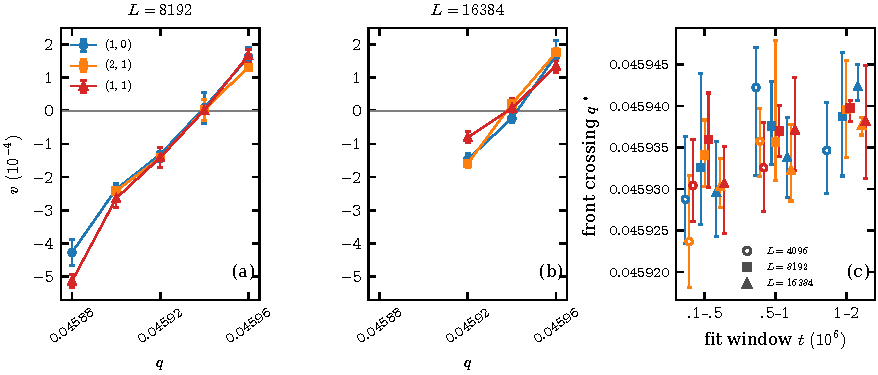
\includegraphics[width=\textwidth]{figs/fig_gpu_fronts}
\caption{Fine-grid front measurements at $p=\alpha=1/2$.
(a,b) Normal velocities at $L=8192$ and $16384$, fitted over
$10^6\le t\le2\times10^6$; four independent bands per point, and bars are
one standard error over runs. The profile threshold is 0.3 of the
reference activity at $t=10^3$. Colors and markers distinguish the three band
normals. Each included group retains a separated pair of fronts throughout
the stated fit window in every run.
(c) Local bracketing estimates of the velocity zero for three successive
windows; colors denote the same normals, while marker shapes denote $L$.
The $L=4096$ groups have eight runs, and the larger sizes four.
Intervals are conditional 95\% run-bootstrap intervals for each chosen
window and threshold. The variation between windows and orientations is
shown separately from sampling uncertainty.}
\label{fig:gpu_fronts}
\end{figure*}

Independent $L=8192$ cohorts followed to $5\times10^6$ steps test the
remaining time dependence (Fig.~\ref{fig:gpu_fronts5m}). For axial bands,
four new runs at each of $q=0.04593$, 0.04594, and 0.04595 give a crossing
of 0.0459340 over $2$--$3.5\times10^6$ and 0.0459435 over
$3.5$--$5\times10^6$. Resampling the same runs in the two windows gives
a paired shift of $9.4\times10^{-6}$ with a conditional 95\% interval
$[4.9,12.1]\times10^{-6}$. The change has the same sign at profile
thresholds 0.2 and 0.5. All fitted bands remain geometrically valid;
at $q=0.04594$, all four interiors retain more than 90\% of the reference
activity at the final time. This is
residual time dependence of an intact front, distinct from the fragmenting
near-voter strips discussed below. It enters the coexistence resolution
rather than being interpreted as demonstrated stationarity.
The local late-window crossings for the diagonal and tilted bands are
0.0459410 and 0.0459390. The diagonal paired change is not resolved.
For tilted bands, one $q=0.04595$ run exceeds the width cutoff at
$t=4.5\times10^6$ with threshold 0.3. The local root remains bracketed
by valid $q=0.04593$ and 0.04594 groups, but the predeclared whole-grid
paired contrast is withheld. At threshold 0.5 all three groups retain
valid geometry and the paired-shift interval includes zero.

\begin{figure*}
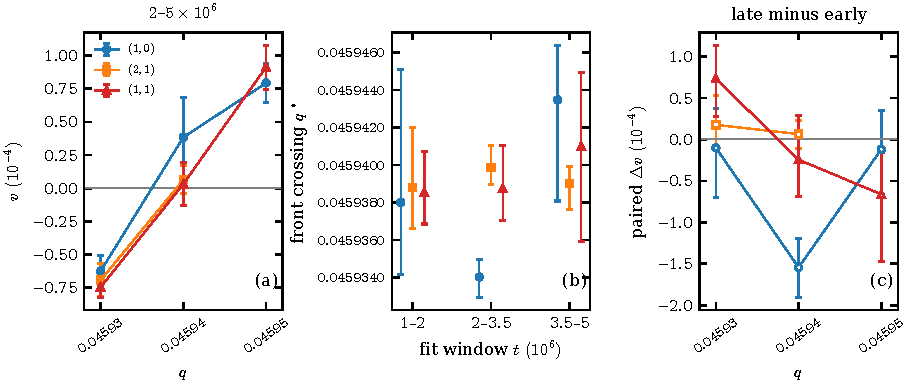
\includegraphics[width=\textwidth]{figs/fig_gpu_fronts5m}
\caption{Independent long-time front test at $p=\alpha=1/2$,
$L=8192$, with four new seeds per $(q,\mathrm{normal})$ and $T=5\times10^6$.
These cohorts are separate from the original $T=2\times10^6$ cohorts.
(a) Normal velocities fitted over $2$--$5\times10^6$, with one standard
error over runs. (b) Local bracketing crossings in successive windows
within the new cohorts, with conditional 95\% run-bootstrap intervals.
(c) Paired differences $v_{3.5\text{--}5\times10^6}-v_{2\text{--}3.5\times10^6}$;
each difference uses the same run in both windows, and bars are 95\%
run-bootstrap intervals. The profile threshold is 0.3. Only complete
predeclared four-seed groups with valid separated-front geometry throughout
both windows contribute. Threshold and interpolation choices remain
separate systematic uncertainties.}
\label{fig:gpu_fronts5m}
\end{figure*}

A further independent axial grid extends the same three probabilities to
$10^7$ steps, again with four new seeds per probability. All twelve runs
retain valid band geometry in both the $2$--$5\times10^6$ and
$5$--$10\times10^6$ windows at all three thresholds. At threshold 0.3,
the local crossing changes from 0.0459372 to 0.0459412; the paired shift
is $4.0\times10^{-6}$ with a conditional 95\% interval
$[2.4,5.6]\times10^{-6}$. The shift remains positive at thresholds 0.2
and 0.5, whose late crossings are 0.0459413 and 0.0459407. The threshold estimator retains residual time dependence in this
independent extension. Its precision is estimator-dependent, as shown
by the integrated-observable comparison below; it does not demonstrate
stationarity. At $q=0.04594$, all four interiors retain more than 90\%
of their reference activity throughout the final window.

For common normalizations below, we adopt the rounded operational reference
$q^*=0.04594$ and vary it over $[0.04592,0.04596]$. This
sensitivity range contains the extended-front point estimates and the
conditional bootstrap intervals reported above; alternative small-sample
intervals can extend beyond it. It is not a pooled confidence interval or a bound
on the limiting coexistence point. The measured time and orientation contrasts
remain part of the physical resolution of the study.

A complementary test places a large droplet of each phase in the other~\cite{wang2015}.
The signs on either side test opposing invasion; shrinkage of both finite
droplets could also be caused by ordinary curvature near a single isotropic zero. Figure~\ref{fig:drop2} shows, at
$p = 1/2$ and $L = 4096$, an active disk of radius 1000 in the dead state and a dead hole of the same
radius in the active state, at $q=0.0456842$, 0.0458221, 0.0460979,
and 0.0462358. At every sampled $q$ one of the two grows
while the other shrinks: above $\qs$ the active disk grows and the hole closes, below $\qs$ the
disk shrinks and the hole opens, with rates compared to a planar-front velocity corrected for
curvature, $\ds R/\ds t = \pm v - D/R$ (Sec.~\ref{M-sec:drops}). The radius estimator and its spatial trimming are specified in
Sec.~\ref{app:numerics}. We compare the corrected growth-law integration
and alternative radius estimators using the same trajectories.
The disk and hole exchange their signs of growth between $q=0.0458221$
and 0.0460979. The primary mean disk rates differ from the integrated
curvature prediction by at most $2.65\times10^{-4}$ sites per step.
For holes the difference is at most $3.60\times10^{-4}$, except at
$q=0.0456842$, where it is $5.78\times10^{-4}$ and the surrounding
metastable active phase also begins to decay. Replacing the trimmed,
rectified area by the full signed area changes the mean hole rate at
$q=0.0458221$ from $0.710\times10^{-3}$ to $0.873\times10^{-3}$,
without changing its sign. The complementary growth signs persist in
every individual run at all four sampled probabilities.

These coarse droplet measurements locate opposing invasion tendencies.
They do not determine whether an asymptotic interval of generic
coexistence lies between the closest points. Even with a single isotropic
front reversal, the curvature law makes both droplets of a finite radius
shrink whenever $|v|<D/R$. Consequently, observing both finite droplets
shrink would also require a radius sequence before it could distinguish
such an interval from ordinary curvature. Here the central droplet gap
is $2.758\times10^{-4}$, well above the observed front-crossing differences.


\begin{figure*}
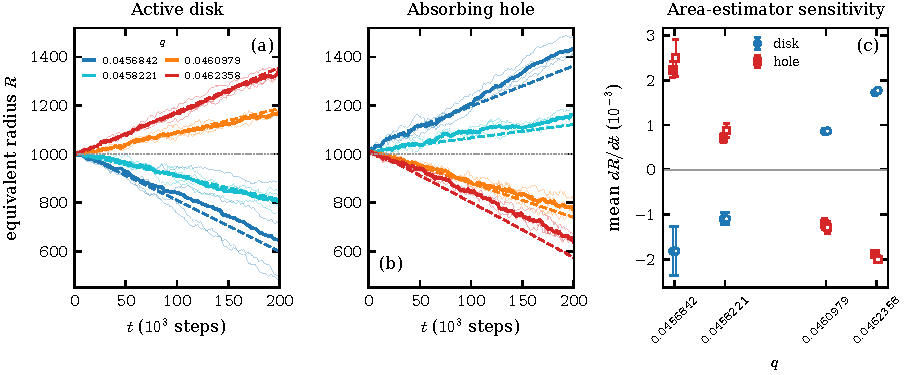
\includegraphics[width=\textwidth]{figs/fig_drop2}
\caption{Complementary droplets at $p=\alpha=1/2$, $L=4096$.
An active disk (a) and an absorbing hole (b) both start with radius 1000.
Thin solid curves show four individual runs per probability and thick
solid curves show their mean equivalent radius. The primary area estimator
uses the trimmed, nonnegative row chords defined in the numerical methods.
Dashed curves integrate $dR/dt=v-D/R$ for disks and $dR/dt=-v-D/R$ for
holes, with $D=0.20$, starting at the measured mean radius at
$t=2\times10^4$. The signed planar velocity $v$ is interpolated at the
actual $q$ from the corrected broad axial-front survey.
(c) Mean radius slopes fitted over $2\times10^4\le t\le2\times10^5$.
Filled markers use the primary trimmed and rectified area, open markers
the full signed area; their small horizontal offsets separate estimators
at the same $q$. Bars are one standard error across four runs.
All individual runs retain the displayed growth or shrinkage sign under
both area definitions.}
\label{fig:drop2}
\end{figure*}


We compare the profile-envelope velocities with slopes of three integrated
observables: twice the live-site fraction, the bond interface density, and
the fraction of sites with a disagreeing neighbor. Their fixed positive
normalizations set equivalent width units but do not move a velocity zero.
At $L=8192$ over $5$--$10\times10^6$ steps, the independent axial cohort
gives crossings 0.04594117, 0.04594063, 0.04594075, and 0.04594075,
respectively. The operational reversal therefore changes little across
these estimators. These observables share the same trajectories and are
not independent confirmations.

At $L=16384$ over $1$--$2\times10^6$ steps, the axial-minus-tilted
crossing difference changes from $4.66\times10^{-6}$ for the envelope
to $2.70\times10^{-6}$ for integrated bond activity. The envelope's
conditional bootstrap contrast excludes zero, while a delta-method
Welch--Satterthwaite sensitivity interval, with Bonferroni adjustment over
three direction pairs, is $[-0.13,9.45]\times10^{-6}$. The apparent angular
separation is thus sensitive to the estimator and small-sample uncertainty
construction. The axial change within the independent $5\times10^6$ cohort
persists across all four observables. For the $10^7$ cohort, the envelope
shift of $4.00\times10^{-6}$ has a delta-method interval
$[1.66,6.34]\times10^{-6}$, whereas the bond-activity shift of
$2.61\times10^{-6}$ has interval $[-0.64,5.85]\times10^{-6}$.
These comparisons support the stated finite-time crossing resolution;
they do not establish a stationary, orientation-independent limit.


